\chapter{Phasen}
\section{Entwurf und Anforderungen}
\subsection{Funktionale Anforderungen}
\begin{itemize}
	\item Das System muss fähig sein zufällig eine Spielwelt mit Hindernissen zu generieren, welche jedoch so platziert werden müssen, dass sie immer überwindbar sind.
	\item Das System muss fähig sein das generierte Spielfeld durch das Bild nach links zu verschieben.
	\item Bei Drücken der Leertaste muss das System die Spielfigur hüpfen lassen.
	\item Das System muss fähig sein einen Highscore in Abhängigkeit zur Spieldauer zu generieren. Der Highscore soll proportional zum Levelfortschritt berechnet werden und dauerhaft angezeigt werden. Hierbei soll der aktuelle Score und der Highscore der Spielesession getrennt angezeigt werden. Dieser wird nur solange gespeichert, bis das Spiel beendet wird.
	\item Das System muss fähig sein während des Spielens eine Hintergrundmusik abzuspielen, welche sich ständig wiederholt.
	\item Das System muss fähig sein beim Springen der Spielfigur, beim Aufkommen der Spielfigur und beim Kollidieren der Spielfigur Effektsounds   wiederzugeben.
	\item Das System muss die Möglichkeit bieten bei Tastendruck das Spiel zu pausieren und wieder zu starten.
	\item Das System muss fähig sein eine Kollision der Spielfigur mit einem Hindernis zu erkennen, nach Erkennen soll ein „Crash“ Sound abgespielt werden und sich die Spielfigur verändern.
	\item Das System muss fähig sein kontinuierlich die Schwierigkeit zu erhöhen. Die Schwierigkeit soll dadurch erhöht werden, dass das Spielfeld anfangs langsam nach links wandert und dies kontinuierlich immer schneller wird.
	\item Bei Beendigung des Spiels muss das System fähig sein das Spiel neu zu starten. 
	\item Das System muss auf einem Gerät mit Tastatur im Browser Chrome ablaufen.
\end{itemize}
\subsection{Nicht funktionale Anforderungen}
\begin{itemize}
	\item Das Spiel sollte intuitiv bedienbar sein.
	\item Die Perfomarnce des Spiels sollte so gut sein, dass keine Frame Einbrüche vorkommen.
	\item Auch auf den weiterverbreiteten Browsern sollte das Spiel spielbar sein.
\end{itemize}
\subsection{Projektplan}
\begin{table}[h]
	\begin{tabular}{l|l}
		\toprule
		\textbf{Datum}& \textbf{Aufgabe}\\
		\midrule
		19.10.2016 & Einführung in jeweilige Projekte der Gruppen 	\\ 
		21.10.2016 & Einführung in jeweilige Projekte der Gruppen	\\
		26.10.2016 & Anforderungen	\\ 
		02.11.2016 & Fertigstellung Präsentation, Ergebnispräsentation der Anforderungen \\
		04.11.2016 & Abgabe der Anforderungsspezifikation via Felix \\
		\bottomrule
	\end{tabular}
	\caption{Phase 1: Entwurf und Anforderungen}
\end{table}
\begin{table}[h]
	\begin{tabular}{l|l}
		\toprule
		\textbf{Datum}& \textbf{Aufgabe}\\
		\midrule
		09.11.2016 & Basis Implementierung 	\\ 
		16.11.2016 & Basis Implementierung + Level Design	\\
		23.11.2016 & Zwischenpräsentation der Implementierung	\\ 
		25.11.2016 & Abgabe: Zwischenstand der Implementation via Felix\\
		30.11.2016 & Level Design Verbesserungen \\
		07.12.2016 & Stabilität \& Bug fixing \\
		14.12.2016 & Ergebnispräsentation der Implementierung \\
		16.12.2016 & Abgabe Implementierungsergebnisses via Felix (Code Freeze) \\
		\bottomrule
	\end{tabular}
	\caption{Phase 2: Implementierung}
\end{table}
\begin{table}[h]
	\begin{tabular}{l|l}
		\toprule
		\textbf{Datum}& \textbf{Aufgabe}\\
		\midrule
		21.12.2016 & Test und Resultate dokumentieren 	\\ 
		11.01.2017 & Ergebnispräsentation	\\
		13.01.2017 & Abgabe der Ergebnisse der Testphase	\\ 
		\bottomrule
	\end{tabular}
	\caption{Phase 3: Test}
\end{table}
\begin{table}[h]
	\begin{tabular}{l|l}
		\toprule
		\textbf{Datum}& \textbf{Aufgabe}\\
		\midrule
		18.01.2017 & Dokumentation 	\\ 
		25.01.2017 & Ergebnispräsentation Dokumentation	\\
		27.01.2017 & Projektvorstellung auf der Projektmesse	\\ 
		\bottomrule
	\end{tabular}
	\caption{Phase 4: Dokumentation und Präsentation}
\end{table}
\newpage
\subsection{Releaseplan}
\begin{longtable}{l|l|p{10cm}}
	\toprule
	\textbf{Version} & \textbf{Datum} & \textbf{Inhalt}\\
	\midrule
	1.0.0 & 09.11.16 & Spiel ist startfähig mit passendem Hintergrund und Spielfigur\\ 
	1.1.0 & 16.11.16 & Automatischer Bildlauf und springen ist möglich\\
	1.2.0 & 30.11.16 & Beinhaltet: Zufallsgenerierte Objekte(Hindernisse) mit unendlichem Level\\ 
	1.3.0 & 07.12.16 & Highscore, Hintergrundlied, Sound beim Springen\\
	1.4.0 & 14.12.16 & Zeitbasierte Geschwindigkeit (Bildlauf)\\
	1.5.0 & 21.12.16 & Erfolgreicher Test mit behobenen Fehlern\\
	\bottomrule
 	\caption{Releaseplan}
\end{longtable}
Beim Releaseplan haben wir uns auf eine Versionierung des Programms mit aufsteigenden Nummern geeinigt. Die Erste Nummer steht hierbei für die Grundlegende Programmversion. Die Zweite für wichtige Updates und die Dritte für Bugfixes zwischendurch. Zur jeweiligen Version haben wir ein Fertigstellungsdatum festgelegt und den dann erforderlichen Inhalt festgelegt.
\newpage
\section{Implementation - Zwischenstand}
\subsection{Erfüllte Anforderungen}
\begin{itemize}
	\item Das System muss fähig sein zufällig eine Spielwelt mit Hindernissen zu generieren welche jedoch so platziert werden müssen dass sie immer überwindbar sind.
	\item Das System muss fähig sein das generierte Spielfeld durch das Bild nach links zu verschieben.
	\item Bei Drücken der Leertaste muss das System die Spielfigur hüpfen lassen.
	\item Das System muss die Möglichkeit bieten bei Tastendruck das Spiel zu pausieren und wieder zu starten.
	\item Das System muss fähig sein kontinuierlich die Schwierigkeit zu erhöhen. Die Schwierigkeit soll dadurch erhöht werden, dass das Spielfeld anfangs langsam nach links wandert und dies kontinuierlich immer schneller wird.
	\item Bei Beendigung des Spiels muss das System fähig sein das Spiel neu zu starten. 
	\item Das System muss auf einem Gerät mit Tastatur im Browser Chrome ablaufen.
\end{itemize}

\subsection{Nicht erfüllte Anforderungen}
\begin{itemize}
	\item Das System muss fähig sein eine Kollision der Spielfigur mit einem Hindernis zu erkennen, nach Erkennen soll ein „Crash“ Sound abgespielt werden und sich die Spielfigur verändern.
	\item Das System muss fähig sein einen Highscore in Abhängigkeit zur Spieldauer zu generieren. Der Highscore soll proportional zum Levelfortschritt berechnet werden und dauerhaft angezeigt werden. Hierbei soll der aktuelle Score und der Highscore der Spielesession getrennt angezeigt werden. Dieser wird nur solange gespeichert, bis das Spiel beendet wird.
	\item Das System muss fähig sein, während des Spielens eine Hintergrundmusik abzuspielen, welche sich ständig wiederholt.
	\item Das System muss fähig sein beim Springen der Spielfigur, beim Aufkommen der Spielfigur und beim Kollidieren der Spielfigur Effektsounds   wiederzugeben.
\end{itemize}
\newpage
\subsection{Das Spiel}
Hier werden zwei Screenshots des derzeitigen Spiels dargestellt. In der Abbildung \ref{pic:start} zu sehen, ist der Startbildschirm des Spiels. Hier gibt es verschiedene Auswahlmöglichkeiten. In der Abbildung \ref{pic:spiel} zu sehen ist der derzeitige Stand des Spiels.
\begin{figure}[htb]
	\centering
	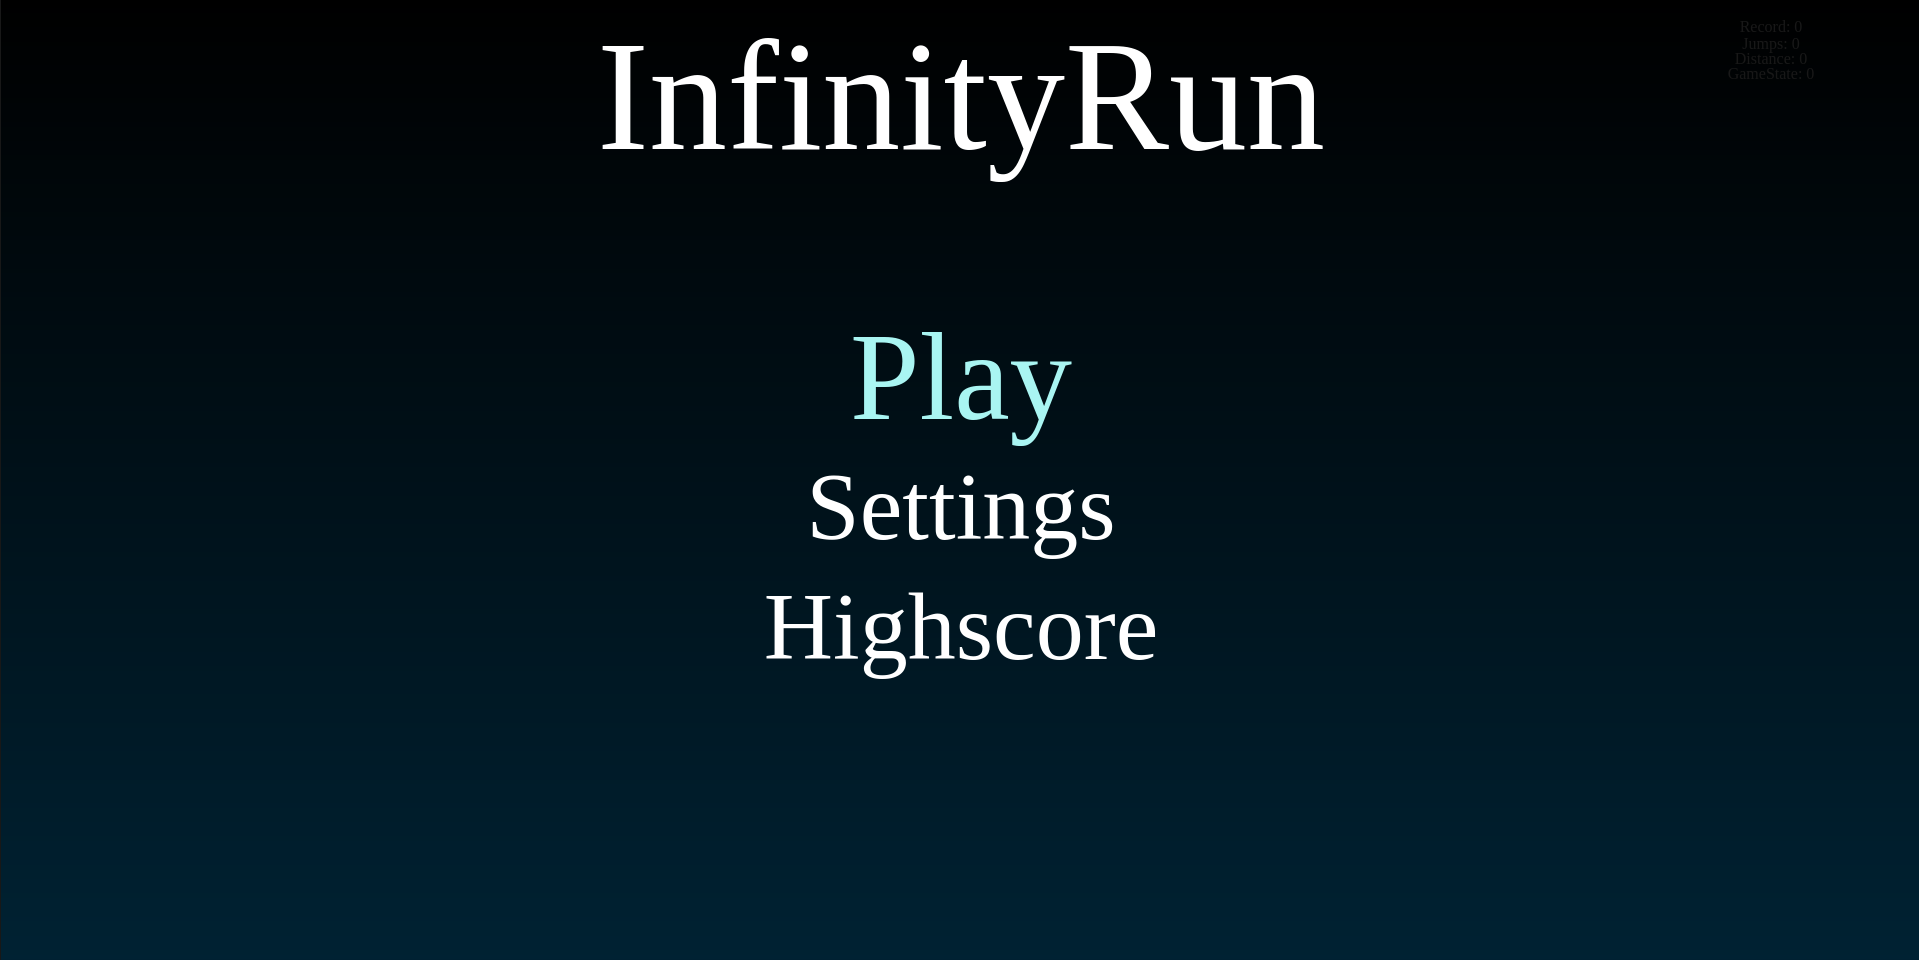
\includegraphics[scale=0.22]{content/pictures/start.png}
	\caption{Startbildschirm}
	\label{pic:start}
\end{figure}
\begin{figure}[htb]
	\centering
	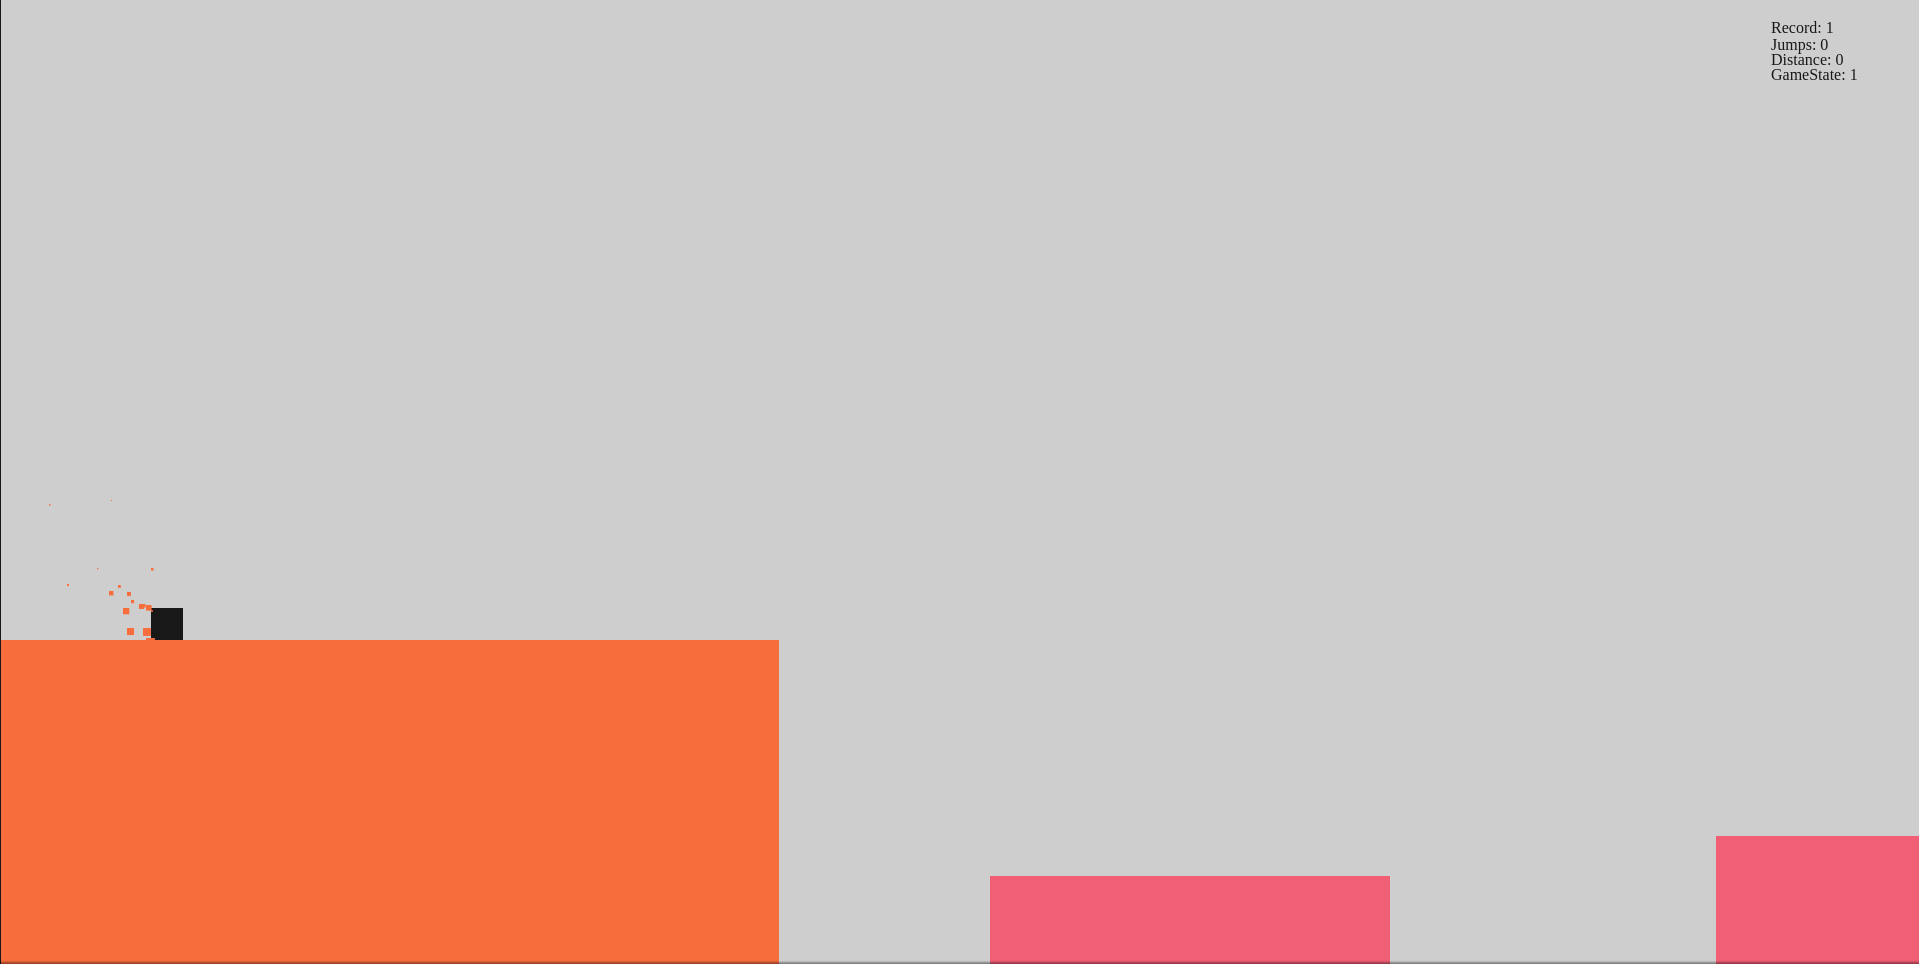
\includegraphics[scale=0.22]{content/pictures/spiel.png}
	\caption{Das Spiel}
	\label{pic:spiel}
\end{figure}
\newpage
\subsection{Bibliothek}
Bei der Erstellung des Spiels greifen wir auf eine JavaScript Bibliothek namens ``Sketch.js'' zurück.
Das Sketch.js Framework ermöglicht es uns, den Code vereinfacht und lesbarer zu schreiben. 
Beispiel wie Sketch.js funktioniert:

\lstset{language=java}
\begin{lstlisting}[frame=single]
function start() 
{
	context.now = +new Date();
    context.running = true;
}
        
function stop() 
{
	context.running = false;
}
        
function toggle() 
{       
	( context.running ? stop : start )();
}
        
function clear() 
{        
	if ( is2D )
        context.clearRect( 0, 0, context.width, context.height );
}
\end{lstlisting}
Quelle: \cite{sketch}
\subsection{Code}
\subsubsection{Framework initialisieren}
Hier in dieser Funktion wird ein Canvas-Element erstellt, dies geschieht mithilfe des Sketch-Frameworks. Dabei werden Eigenschaften wie die H\"ohe und Breite der Zeichenfl\"ache \"ubergeben.
\lstset{language=java}
\begin{lstlisting}[frame=single]
var InfinityRun = Sketch.create({
fullscreen: true,
width: 640,
height: 360,
container: document.getElementById('container')
});
\end{lstlisting}
\subsubsection{Spieler initialisieren}
In der Player-Update-Funktion wird der Player also unsere Spielfigur aktualisiert. Damit die Schwerkraft gegeben ist, wird zuerst die Y-Geschwindigkeit um eins erhöht. Hierbei ist zu beachten, dass die Y- Koordinatenachse nach unten zeigt.Danach wird die Position des Spielers neu festgesetzt. Für den Fall, dass der Spieler verliert, welches mittels if-Entscheidung überprüft wird, werden dann anschließend sämtliche Spielwerte auf ihren Ausgangswert zurückgesetzt. Als letztes wird überprüft ob der Spieler eine Taste gedrückt um zu Springen. Falls ja und er sich nicht schon in der Luft befindet wird die Y-Geschwindigkeit in die negative Richtung erhöht und die Spielfigur springt.
\lstset{language=java}
\begin{lstlisting}[frame=single]
Player.prototype.update = function() {
// Gravity 
this.velocityY += 1;
this.setPosition(this.x + this.velocityX, this.y + this.velocityY);

if (this.y > InfinityRun.height || this.x + this.width < 0) 
{
	this.x = 150;
	this.y = 50;
	this.velocityX = 0;
	this.velocityY = 0;
	InfinityRun.jumpCount = 0;
	InfinityRun.acceleration = 0;
	InfinityRun.accelerationTweening = 0;
	InfinityRun.scoreColor = '#181818';
	InfinityRun.platformManager.maxDistanceBetween = 350;
	InfinityRun.platformManager.updateWhenLose();
}

if ((InfinityRun.keys.UP || InfinityRun.keys.SPACE || InfinityRun.keys.W || InfinityRun.dragging) && this.velocityY < -8) 
{
	this.velocityY += -0.75;
}
};
\end{lstlisting}
\subsubsection{Erstellen der Spielebene}
In unserem Plattform-Manager werden die Plattformen initialisiert. Hierbei wird ein Wert ''maxDistanceBetween'' festgelegt. Ebenso werden mögliche Farben für die Plattformen gespeichert. Anschließend werden den ersten 3 Plattformen ihre Werte zugeordnet. Die erste Plattform hat hierbei feste Werte, damit der Spieler nicht sterben kann, am Anfang des Spiels. Die beiden nächsten Plattformen werden dann mit zufälligen Werten erstellt. Zum Schluss bekommt jede Plattform noch eine Höhe und Farbe zugeordnet.
\lstset{language=java}
\begin{lstlisting}[frame=single]
Player.prototype.update = function() {
function PlatformManager() 
{

	this.maxDistanceBetween = 300;

	this.colors = ['#2ca8c2', '#98cb4a', '#f76d3c', '#f15f74', '#5481e6'];

//first 3 Platforms execept the Starter Platform
	this.first = new Platform({
	x: 300,
	y: InfinityRun.width / 2,
	width: 400,
	height: 70
})

this.second = new Platform
({
	x: (this.first.x + this.first.width) + random(this.maxDistanceBetween - 150, this.maxDistanceBetween),
	y: random(this.first.y - 128, InfinityRun.height - 80),
	width: 400,
	height: 70
})

this.third = new Platform
({
	x: (this.second.x + this.second.width) + random(this.maxDistanceBetween - 150, this.maxDistanceBetween),
	y: random(this.second.y - 128, InfinityRun.height - 80),
	width: 400,
	height: 70
})
	this.first.height = this.first.y + InfinityRun.height;
	this.second.height = this.second.y + InfinityRun.height;
	this.third.height = this.third.y + InfinityRun.height;
	this.first.color = randomChoice(this.colors);
	this.second.color = randomChoice(this.colors);
	this.third.color = randomChoice(this.colors);
	this.colliding = false;
	this.platforms = [this.first, this.second, this.third];
}
\end{lstlisting}
\subsubsection{Update der Plattformen}
Die Plattform-Update-Funktion aktualisiert die 3 Plattformen. Sie hat zwei Aufgaben. Als erstes wird die Plattform immer, in Abhängigkeit zur Spielbeschleunigung, nach um drei nach links verschoben. Danach wird abgefragt, ob die Plattform schon ganz links aus dem Bild heraus gewandert ist und falls ja werden sämtliche Werte so zufällig neu gesetzt, dass sie wieder von rechts ins Bild laufen kann. Dies wird für alle 3 Plattformen gleich durchgeführt.
\lstset{language=java}
\begin{lstlisting}[frame=single]
PlatformManager.prototype.update = function() 
{
	this.first.x -= 3 + InfinityRun.acceleration;
	if (this.first.x + this.first.width < 0) 
	{
		this.first.width = random(450, InfinityRun.width + 200);
		this.first.x = (this.third.x + this.third.width) + random(this.maxDistanceBetween - 150, this.maxDistanceBetween);
		this.first.y = random(this.third.y - 32, InfinityRun.height - 80);
		this.first.height = this.first.y + InfinityRun.height + 10;
		this.first.color = randomChoice(this.colors);
	}

	this.second.x -= 3 + InfinityRun.acceleration;
	if (this.second.x + this.second.width < 0) 
	{
		this.second.width = random(450, InfinityRun.width + 200);
		this.second.x = (this.first.x + this.first.width) + random(this.maxDistanceBetween - 150, this.maxDistanceBetween);
		this.second.y = random(this.first.y - 32, InfinityRun.height - 80);
		this.second.height = this.second.y + InfinityRun.height + 10;
		this.second.color = randomChoice(this.colors);
	}

	this.third.x -= 3 + InfinityRun.acceleration;
	if (this.third.x + this.third.width < 0) 
	{
		this.third.width = random(450, InfinityRun.width + 200);
		this.third.x = (this.second.x + this.second.width) + random(this.maxDistanceBetween - 150, this.maxDistanceBetween);
		this.third.y = random(this.second.y - 32, InfinityRun.height - 80);
		this.third.height = this.third.y + InfinityRun.height + 10;
		this.third.color = randomChoice(this.colors);
	}
};
\end{lstlisting}
\subsubsection{Update der Plattformen}
In folgender Funktion werden mithilfe einer for-Schleife zuerst alle drei Plattformen abgefragt, ob diese, anhand von: "if(this.player.intersects..) " den Spieler ber\"uhren. Falls der Spieler eine Plattform ber\"uhrt, in diesem Fall " this.collidedPlatform.... " als Beispiel die zweite Plattform im Spiel ber\"uhrt, so wird der Variable "collidedPlatform" ein Objekt der zweiten Plattform zugewiesen. Außerdem wird zus\"atzlich noch die Y-Koordinate des Spielers auf die der Plattform gesetzt, was hier die Funktion " this.player.y < this.platformManager...." ist. Zus\"atzlich wird wenn die Y-Koordinate des Spielers und die Y-Koordinate der Plattform \"ubereinstimmen, die "velocityY" auf 0 gesetzt, was zur Folge hat, dass der Spieler nicht mehr f\"allt. Anschließend sollen die Partikel des Spielers die Farbe der Plattormen annehmen.
\lstset{language=java}
\begin{lstlisting}[frame=single]
    for (i = 0; i < this.platformManager.platforms.length; i++) 
    {
		if (this.player.intersects(this.platformManager.platforms[i])) 
		{
			this.collidedPlatform = this.platformManager.platforms[i];
			if (this.player.y < this.platformManager.platforms[i].y) 
			{
				this.player.y = this.platformManager.platforms[i].y;
				// Gravity after Collision with Platform
				this.player.velocityY = 0;
			}

			this.player.x = this.player.previousX;
			this.player.y = this.player.previousY;
			
			this.particles[(this.particlesIndex++) % this.particlesMax] = new Particle({
			x: this.player.x,
			y: this.player.y + this.player.height,
			color: this.collidedPlatform.color
});
\end{lstlisting}
\subsection{Nächste Ziele}
Da die Grundlegenden Spielfunktionen implementiert sind wollen wir uns in der zweiten Phase der Implementation nun auf das Design und die Effektsounds konzentrieren.
\section{Implementation - Endstand}
\subsection{Spielkonzept Änderungen}
Folgende Spielkonzept Äbnderungen haben wir im laufe der Implementation vorgenommen:
\begin{itemize}
	\item Die Spielebene hat anstatt Hindernisse Zufalls generierte variable Plattformen.
	\item Spiel-Menü eingefügt
	\item Spielhintergrund
\end{itemize}
\subsection{Funktionsdiagramm}
\subsection{Grafiken}
\subsection{Sounds}
Bei den implementierten Spielsounds greifen wir auf eine freie Sounddatenbank zurück. Quelle: \cite{sounds}\\
Folgende Sounds werden wir verwenden:
\begin{table}[h]
	\centering
	\begin{tabular}{|l|l|}
		\toprule
		\textbf{Sounds}& \textbf{Links}\\
		\midrule
		Menu & \url{https://www.freesound.org/people/lharman94/sounds/329597/}\\ 
		Main1 & \url{https://www.freesound.org/people/nicolasdrweski/sounds/179684/}\\
		Main2  & \url{https://www.freesound.org/people/joshuaempyre/sounds/251461/}\\ 
		Main3  & \url{https://www.freesound.org/people/Flick3r/sounds/48544/}\\
		Main4 & \url{https://www.freesound.org/people/Flick3r/sounds/45623/}\\
		Jump & \url{https://www.freesound.org/people/Lefty_Studios/sounds/369515/}\\
		Level-Up & \url{https://www.freesound.org/people/n_audioman/sounds/275895/}\\
		Error & \url{https://www.freesound.org/people/SamsterBirdies/sounds/363920/}\\
		Crash & \url{https://www.freesound.org/people/n_audioman/sounds/276341/}\\
		\bottomrule
	\end{tabular}
	\caption{Sound Links}
\end{table}
\section{Test}
\section{Dokumentation \& Pr\"asentation}

